\documentclass{catalogue}

\title{Aufgabenkatalog fürs Aufwärmen}

\begin{document}
    \Large
    \maketitle

    \begin{figure}
        
\includegraphics[width=0.9\linewidth]{src/images/RZZ_Logo.png}
        \label{fig:RZZ_Logo}
    \end{figure}
    \newpage

    \section{Kreislauf}
        1 Suche eine Übung aus, 5-10 min 

    \subsection{Joggen}
    \begin{minipage}{0.34\linewidth}
        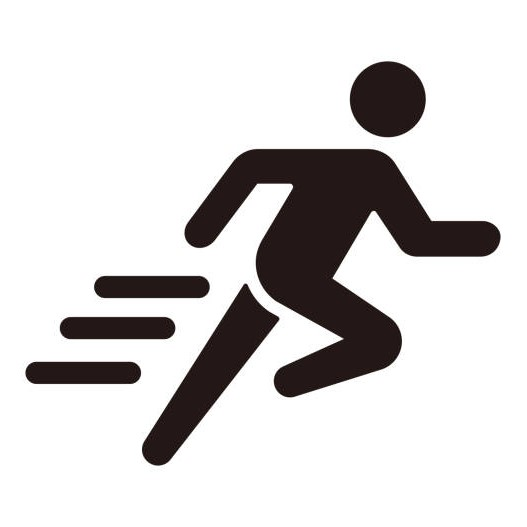
\includegraphics[width = \linewidth]{src/1_kreislauf/images/joggen_piktogramm.jpg}
    \end{minipage}
    \begin{minipage}{0.64\linewidth}
        \begin{itemize}
            \item 5-10 Minuten Joggen
            \item 3x 1 Min Sprint + 1 Min locker
            \item 30s Sprungvarianten einbauen
        \end{itemize}
    \end{minipage}

    \subsection{Seilspringen}
    \begin{minipage}{0.34\linewidth}
        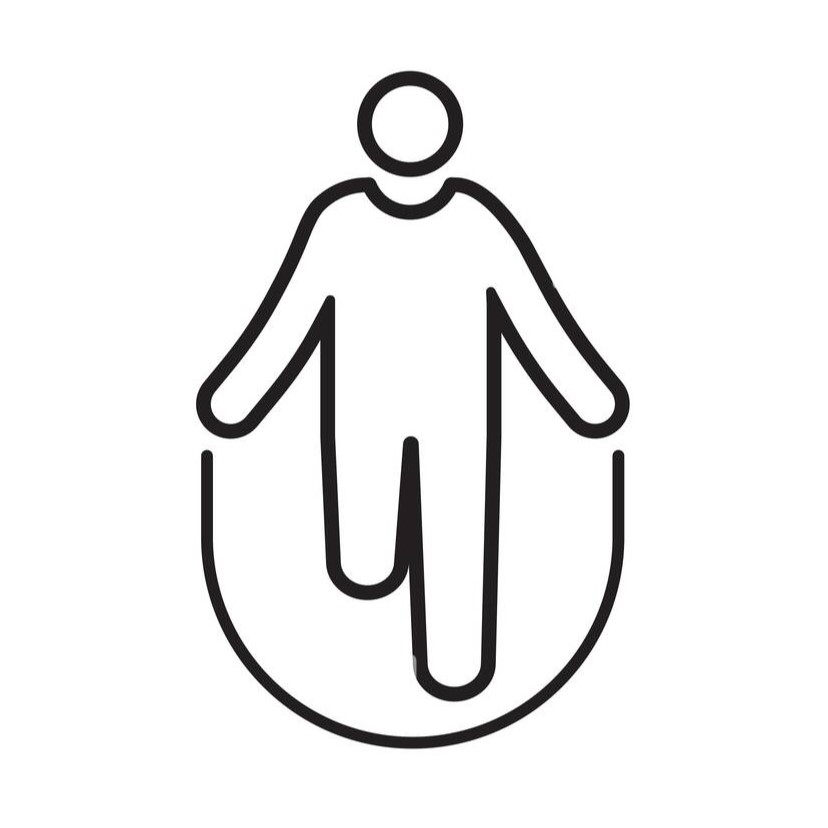
\includegraphics[width = \linewidth]{src/1_kreislauf/images/seilspringen_piktogramm.jpg}
    \end{minipage}
    \begin{minipage}{0.64\linewidth}
        \begin{itemize}
            \item 
        \end{itemize}
    \end{minipage}

\begin{itemize}
    \item Seilspringen
    \item Treppenlaufen
\end{itemize}
        \newpage
    
    \section{Mobilisieren}
        Suche 4-5 Übungen aus, 10 Wiederholungen je
\begin{itemize}
    \item Kopf / Nacken
    \item Schultern
    \item Ellenbogen
    \item Handgelenke
    \item Finger
    \item Hüfte
    \item Knie
    \item Fussgelenk
\end{itemize}
        \newpage

    \section{Eindehnen}
        Suche einen Ablauf aus, halte jede Position mind. 5 Sekunden.
\begin{itemize}
    \item Flow auf Bauch und Rücken
    \item Flow Stütz
    \item Flow Spagat und seitlicher Schritt
\end{itemize}
        \newpage
    
    \section{Aktivieren}
        Suche 4 Übungen aus
\begin{itemize}
    \item Burpees
    \item Beine
    \item Arme
    \item Rumpf
    \item Schnellkraft
    \item Maxkraft
\end{itemize}
        \newpage

    \section{Spezifische Übungen}
        \begin{itemize}
    \item 2 Toppasrouten
    \item Traverse an Boulderwand
    \item 10 einfache Boulders (bis B3)
    \item 5 Minuten an einfachen Griffen Kreiseln
\end{itemize}
\end{document}